\section{CountMax的系统集成测试}\label{sec:proto}

为了验证CountMax的可行性,我们基于Open vSwitch软交换机开发了一个原型系统,并测试了我们的sketch。

\subsection{测试指标与基准}\label{sec:testbedmetric}
系统测试中我们采用了3种不同的指标。其中之一是最大链路负载率,在第\ref{subsec:metric}小节中已经定义。另外两种如下:
\begin{enumerate}
	\item
    处理一个包所需的平均CPU时钟周期数。
    第\ref{sec:simulation}节中所述的运行时间会被主机上的其他因素,如代码JIT编译、后台进程等所影响,因此我们采用CPU周期来衡量系统测试中的计算负载\cite{huang2017sketchvisor}。
    通过在sketch代码中插入查询CPU计数器的API,我们可以得到处理一个数据包所需的平均CPU时钟周期数。
	\item
    Sketch每秒可处理的数据包数(pps),即吞吐量。我们一次性发送巨大数量的数据包,来测试在占满计算资源的情况下,sketch的处理能力。
\end{enumerate}


\subsection{系统实现与设置}
\begin{figure}[ht]
	\centering
	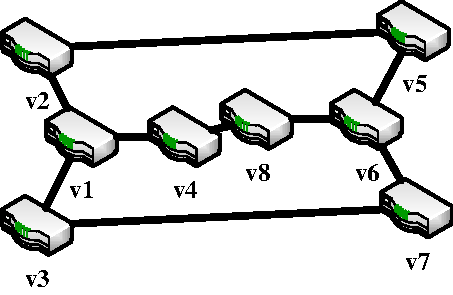
\includegraphics[width=0.68\linewidth]{fig/topo.pdf}
	\caption{\textnormal{系统测试的拓扑。}}
	\label{fig:prototypetopo}
	\note{$v_3,v_4,v_5,v_6$ 分别连接了一个主机。图中未画出控制器和主机。}
\end{figure}

图\ref{fig:prototypetopo}示意了系统测试所用的拓扑。
拓扑中包含一个控制器,6个虚拟交换机,以及4个主机。出于简洁起见,图中没有画出控制器和主机。
控制器使用Ryu \cite{ryu}实现。虚拟交换机基于Open vSwitch (OVS)2.8.2版本\cite{openvswitch}。主机为虚拟主机。
交换机3~6上集成了sketch,并且它们的sketch只处理入站流量。

我们使用C语言实现了CountMax、CountSketch和FSS,使用gcc编译器\cite{gcc}的-O2选项进行优化,并将它们分别集成到OVS的datapath内核模块中。
在OVS处理到达的数据包时,它将会调用sketch来进行更新操作。
sketch监听一个TCP端口用来上报自己的统计数据。

重路由测试的方式与第\ref{sec:simulation}节相似。
在所有的流都处理完毕后,收集sketch的统计数据进行脱机计算。
将计算得出的路由作为流表下发到交换机中,然后再次发送这些流。
通过OVS所搭载的端口统计功能获取链路负载信息。

CPU周期测试的形式为预先生成好大量的伪数据包,将它们的信息直接提供给一个单独的sketch实例,此过程中没有产生实际的网络流量。

CPU周期测试运行在Windows 10操作系统上,其他的测试则运行在Ubuntu 14.04 LTS,Linux内核版本4.10。

集成了CountMax的OVS内核模块的代码公布在https://github.com/VALLIS-NERIA/ovs-datapath。
 
\subsection{测试结果}

\begin{figure}[!t]
	\centering
	\begin{minipage}[t]{0.48\linewidth}		
		%\begin{figure}[!t]
		\centering
		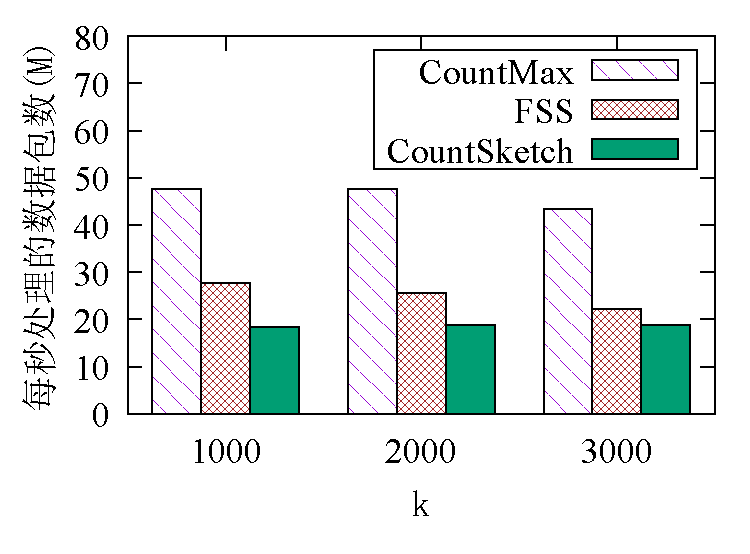
\includegraphics[width=\linewidth]{fig/throughput.pdf}
		\caption{\textnormal{不同sketch的吞吐量随$k$变化。}}
		\label{fig:prototype,bandwidth}
		%\end{figure}
	\end{minipage}\vspace{-0.6em}\hspace{0.4em}
	\begin{minipage}[t]{0.48\linewidth}
	\centering
        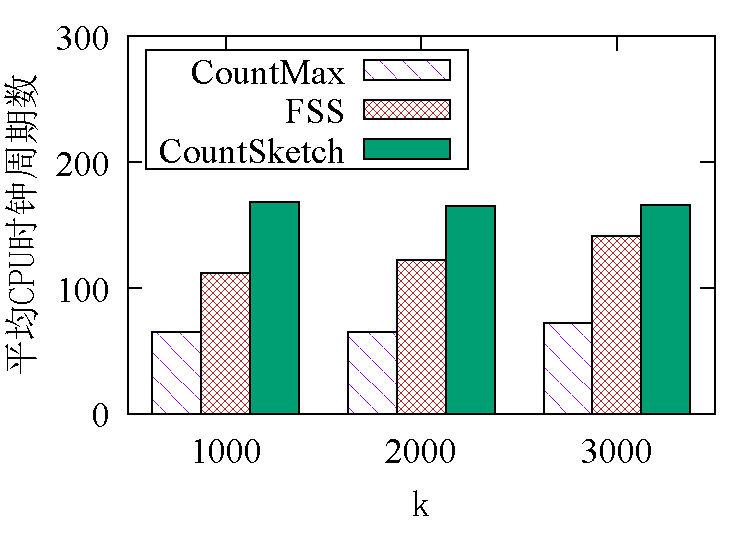
\includegraphics[width=\linewidth]{fig/k_cpu_2000.pdf}
        \caption{\textnormal{处理数据包的平均CPU周期。}}
        \label{fig:prototype,cycle}
	\end{minipage}\vspace{-0.6em}
\end{figure}


\begin{figure}[!t]
	\centering
	\begin{minipage}[t]{0.48\linewidth}		
		%\begin{figure}[!t]
		\centering
		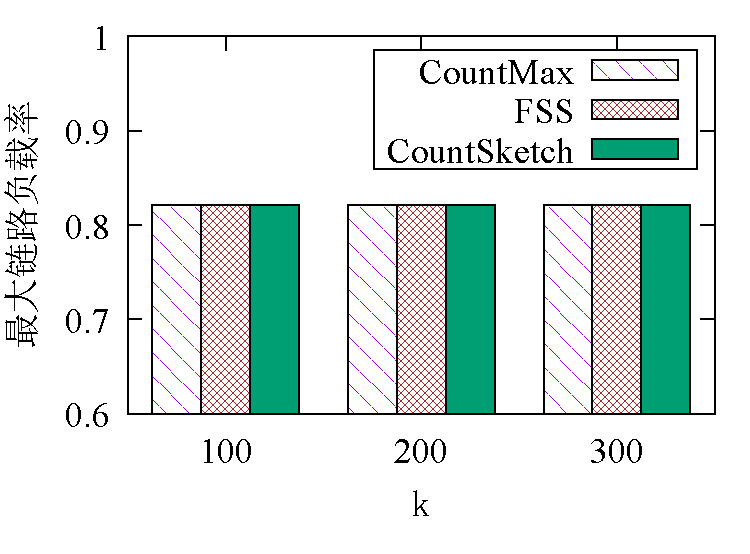
\includegraphics[width=\linewidth]{fig/proto_k_load_2000.pdf}
		\caption{\textnormal{最大链路负载与$k$,2000条流。}}
		\label{fig:prototype,load,k}
		%\end{figure}
	\end{minipage}\vspace{-0.6em}\hspace{0.4em}
	\begin{minipage}[t]{0.48\linewidth}
		\centering
		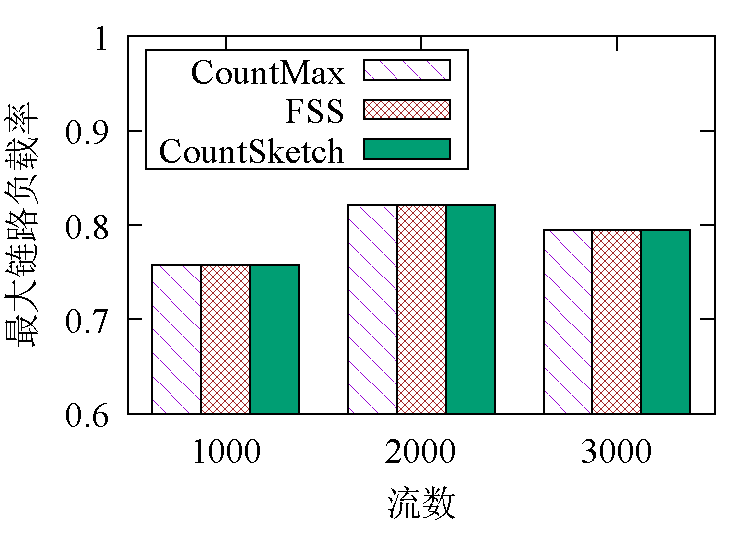
\includegraphics[width=\linewidth]{fig/proto_flow_load_200.pdf}
		\caption{\textnormal{最大链路负载与流数,$k=100$。}}
		\label{fig:prototype,load,flow}
	\end{minipage}\vspace{-0.6em}
\end{figure}


%Figs. \ref{fig:prototype,bandwidth} and \ref{fig:prototype,cycle} are about the computing overhead evaluation.
图\ref{fig:prototype,bandwidth} 体现了不同sketch的吞吐率。
最初我们将sketch装载到一个单独的OVS实例上,并对它进行压力测试,结果发现sketch对于吞吐率的影响不到1\%。
经过深入研究,我们发现OVS作为软交换机,绝大多数的计算资源都被用来和物理网卡进行数据交换以及流表的匹配,sketch占用的计算资源显得微不足道。
而在实体交换机中,流表匹配和包的转发由专用芯片进行处理,sketch的计算负载并不是微不足道的。
因此最终我们将sketch抽离出来,使用生成的数据包单独进行压力测试。
图\ref{fig:prototype,bandwidth}显示,在我们的测试平台下,CountMax、FSS和CountSketch每秒分别可以处理50M、30M和20M个数据包。

在CPU测试当中,每组测试运行了10次以尽可能消除误差。图\ref{fig:prototype,cycle}显示CountMax、FSS、CountSketch处理每个数据包分别需要60、110、170个时钟周期。
代入第\ref{sec:observation}节的假设,计算可得CountMax、FSS、CountSketch将会分别消耗26\%、44\%和68\%的CPU时间。
当网络负载变重,如$\beta=0.6$时,CountMax会消耗约72\%的CPU时间,而FSS和CountSketch则会消耗132\% 和 204\%的CPU时间。
后两者的数字超过了100\%,这意味着统计数据可能会出现丢失的情况,交换机上的其它功能可能无法正常运行。
对于CountMax而言,交换机上的其它功能仍有可能能够正常运行。
与前一节中的图\ref{fig:time,k}相比,这一组测试中CountMax与另两种sketch的计算负载的差距没有那么显著。
其原因在于系统测试使用的是C语言实现,启用了优化,且其中用到的数据结构是专门编写的;
而仿真模拟中使用的是编译成中间代码的C\#语言,没有开启优化,且用到的哈希堆是由系统库中通用的哈希表和小根堆拼凑而成的。
另外,系统测试中的$k$的规模也远小于仿真模拟中的$k$,因而$O(\log{k})$的时间复杂度显示的不明显。

图\ref{fig:prototype,load,k} 和图 \ref{fig:prototype,load,flow}是关于重路由性能的。
从中可以看到$k=100$即可处理2000条流,而随着流数的增加,链路负载也在增加。
总体上结果与第\ref{sec:simulation}节中的结果类似,3种sketch在重路由的方面性能几乎一致。

系统测试的结果显示,CountMax消耗的CPU计算资源分别比FSS和CountSketch少约40\%和60\%,而在应用于重路由方面时,三者的性能几乎完全相同。
因而,CountMax在没有牺牲重路由性能的前提下,降低了处理数据包的计算负载。
